%%%%%%%%%%%%%%%%%%%%%%%%%%%%%%%%%%%%%%%%%%%%%%%%%%%%%%%%%%%%%%%%%%%%%%%%%%%%%%%%%%%
%%                          Document Setup & Headings                            %%
%%%%%%%%%%%%%%%%%%%%%%%%%%%%%%%%%%%%%%%%%%%%%%%%%%%%%%%%%%%%%%%%%%%%%%%%%%%%%%%%%%%
\documentclass{ipfwpaper}
\svnid{$Id$}

% Authors Names and Emails
\author{Paul TREHIOU \formatemail{paul.trahiou@utbm.fr} \\ Victor SENE \formatemail{victor.sene@utbm.fr}}  

\title{TP1 - Introduction à l'AOSP}  % Rename with project title
\course{LO52}  %%%%% Update Course # here
\pagecolor{white}

%%%%%%%%%%%%%%%%%%%%%%%%%%%%%%%%%%%%%%%%%%%%%%%%%%%%%%%%%%%%%%%%%%%%%%%%%%%%%%%%%%%
%%                                 Use Packages                                  %%
\usepackage[utf8]{inputenc}
\usepackage{enumitem,amssymb}
\usepackage{colortbl}
\usepackage{float}
\usepackage{caption}
\usepackage{graphicx}
\usepackage{pdfpages}
\usepackage{gensymb}
\usepackage[acronym,smallcaps]{glossaries}
\usepackage{multicol}
\usepackage{multirow}
%\usepackage[table]{xcolor}
\usepackage{listings}
\usepackage{url}
%%%%%%%%%%%%%%%%%%%%%%%%%%%%%%%%%%%%%%%%%%%%%%%%%%%%%%%%%%%%%%%%%%%%%%%%%%%%%%%%%%%
\usepackage{hyperref} % must be last package loaded!
% it makes hyper-references (citations, URLs, etc) clickable
%%%%%%%%%%%%%%%%%%%%%%%%%%%%%%%%%%%%%%%%%%%%%%%%%%%%%%%%%%%%%%%%%%%%%%%%%%%%%%%%%%%

\definecolor{mygreen}{rgb}{0,0.6,0}
\definecolor{mygray}{rgb}{0.5,0.5,0.5}
\definecolor{mymauve}{rgb}{0.58,0,0.82}

\lstset{ %
  language=Java,                   % language par défaut
  backgroundcolor=\color{white},   % choose the background color
  breaklines=true,                 % automatic line breaking only at whitespace
  captionpos=b,                    % sets the caption-position to bottom
  commentstyle=\color{mygreen},    % comment style
  escapeinside={\%*}{*)},          % if you want to add LaTeX within your code
  keywordstyle=\color{blue},       % keyword style
  stringstyle=\color{mymauve},     % string literal style
}

\begin{document} % this tells the compiler that it is time to make text to print instead of just getting ready.
\maketitle  % make a title page from the Title, Date, and Author
\newpage

%%%%%% Table of Contents %%%%%%

%\section{List of Figures}
		\listoffigures
%	\section{List of Tables}
		\listoftables
\tableofcontents % make a table of contents
\newpage
\section{Initialisation environnement de développement}
Pour commencer, nous avons réalisé l'installation des outils nécessaires au développement d'application Android. Paul a installé Android Studio et Victor a installé le module complémentaire Android dans Intellij IDEA.

\begin{center}
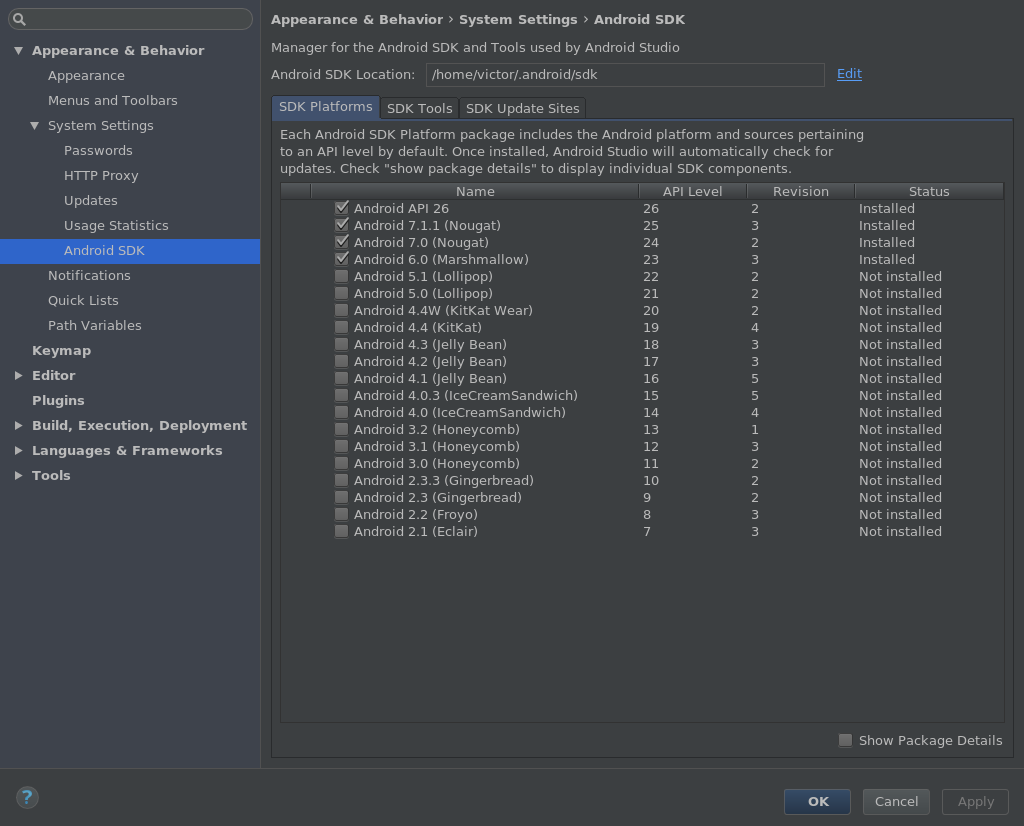
\includegraphics[height=13cm]{img/screenshot_sdk.png}
\end{center}

L'installation des compléments Android a prit beaucoup de temps mais est très guidé et l'IDE réalise le téléchargement de tous les composants nécessaires.
Nous avons ensuite initialisé un dépôt git et créé une nouvelle branche nommé "star lord".
Afin de faciliter l'authentification, nous avons ajouté nos clés SSH à nos comptes Github.

\begin{center}
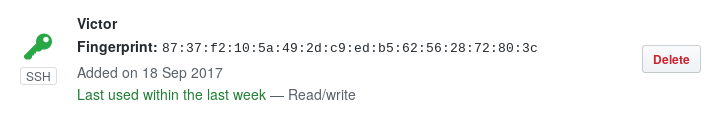
\includegraphics[height=2.5cm]{img/screenshot_ssh.png}
\end{center}

Pour aller plus loin de l'utilisation de Github et apprendre à gérer plusieurs repository en même temps, nous avons créé un repo miroir et ajouté la branche en tant que remote supplémentaire.
\begin{lstlisting}
git remote add origin git@github.com:Vskilet/lo52.git master
\end{lstlisting}

\section{Première application}
Pour reprendre un peu les bases du développement Android, nous avons suivi à la lettre le tutoriel \href{https://developer.android.com/training/basics/firstapp/index.html}{"Build Your first App"}. Les étapes principales consistent en à la création d'une activité principale puis d'envoyer un message sur une seconde activité. Nous avons aussi réussi à faire réagir un bouton lorsqu'on clique sur un bouton grâce à l'attribut "onClick" de la plupart des objets Java pour Android. 

\begin{center}
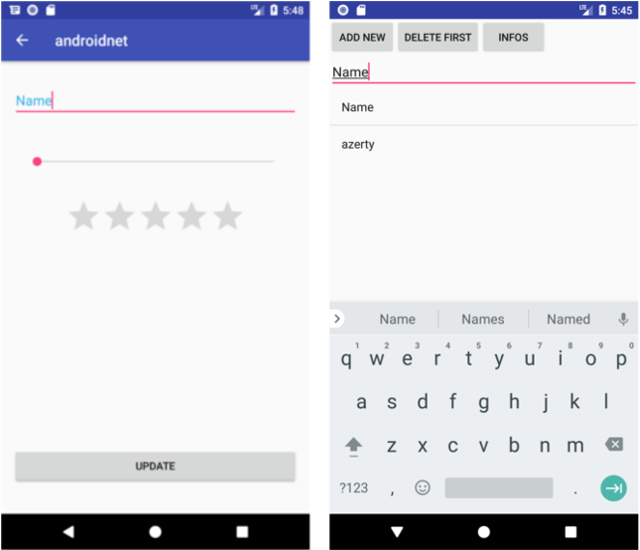
\includegraphics[height=6cm]{img/androidsqlitedatabase.png}
\end{center}

Après avoir créé la seconde activité, nous avons réfléchi à la structure de la base de donnée et graphique de notre application. Nous sommes arrivés à la conclusion, après quelques recherches, que nous devions utiliser les Rooms pour gérer notre base de donnée mais nous développeront l'utilisation dans un rapport ultérieur. Nous aborderons aussi comment nous avons initialisé notre base avec un fichier .db contenant l'ensemble des informations utiles pour la vente de volant.

\section{Base de donnée}
Pour notre base, il s'agit principalement de stocker des informations sur des volants puis de gérer un stock. Nous avons donc une base contenant les Tubes de volant avec leur marque, prix, référence, ...
Pour avoir un historique des achats et ainsi suivre les stocks, nous avons ajouté une base Vente. Une dernière base regroupe les différentes marques de volant afin de facilité le choix lorsque l'on ajoutera un volant à notre liste évolutive.

\begin{center}
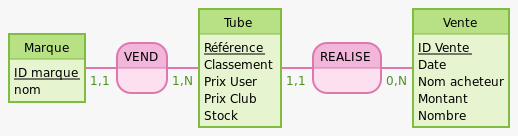
\includegraphics[height=3cm]{img/MCD_Tubes_2.png}
\end{center}
\section{Conclusion}
Finalement ce TP nous a donné envie d'aller plus loin dans le développement et en se prenant au jeu nous avons cherché des bonnes pratiques sur internet pour faire une "bonne" application. Cependant nous avons aussi été un peu freinés par la complexité de la mise en place de composant qui peuvent paraître basique comme un bouton cliquable qui envoie des informations à une activité ... 
\section{Code source}
\url{https://github.com/gxfab/LO52_A2017/tree/b2fca85bbb2e08ce8461b6c335ce18ed48f0cd2c/star_lord}
\end{document}
